\textbf{\underline{OZ 4 - De wet van Ampère en de wet van Biot-Savart - Oefening 1:}}
\vspace{0.5cm}

Een geleider bestaat uit een cirkelvormige lus met straal $R$ en twee lange rechte stukken. De draad ligt in het vlak van het blad en er loopt een stroom $I$ doorheen. Bepaal de grootte en de richting van het magnetische veld dat geproduceerd wordt in het centrum van de lus.

\begin{center}
    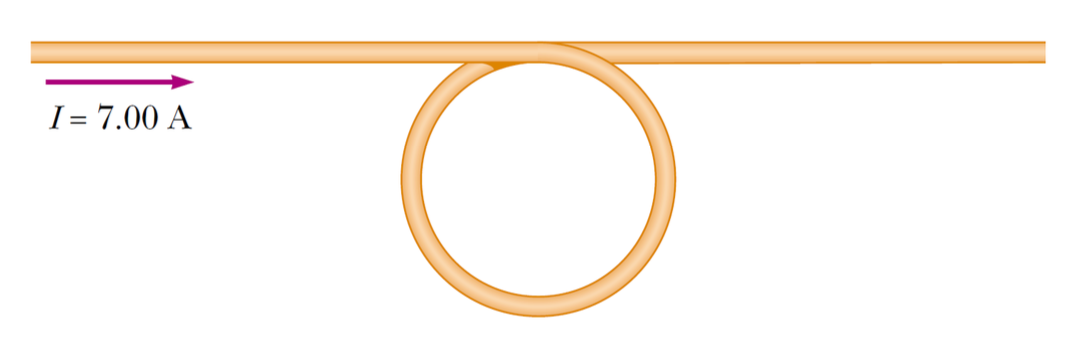
\includegraphics[scale = 0.5]{oz04/resources/Oz4Oef1.png}
\end{center}

\begin{description}[labelwidth=1.5cm, leftmargin=!]
    \item[Geg. :]   $I = 7.00$A, $R$
    \item[Gevr. :]  $\Vec{B}$ ?
    \item[Opl. :]  
    Stel nu dat $d\ell$ een infinitesimaal deeltje cirkelboog, dan is het infinitesimaal magnetisch veld door de lus
    \begin{align*}
        dB_L
            &= \frac{\mu_0I}{4\pi}\frac{d\ell}{R^2} \\
            &= \frac{\mu_0I}{4\pi}\frac{\sin(\gamma)}{R}d\theta \\
            &\overset{\perp}{=} \frac{\mu_0I}{4\pi}\frac{d\theta}{R} 
    \end{align*}
    waarbij $\gamma$ de hoek is tussen $\Vec{r}$ en $d\Vec{\ell}$ hierover integreren om het totale magnetische veld te bekomen
    \begin{align*}
        B_L
            &= \int_{0}^{2\pi} \frac{\mu_0I}{4\pi}\frac{d\theta}{R}  \\
            &= \frac{\mu_0I}{4\pi R} \int_{0}^{2\pi}d\theta \\
            &=  \frac{\mu_0I}{2R}
    \end{align*}
    Het bovenste punt zou twee keer moeten meegeteld worden, omdat er een overlap is loodrecht boven het punt. Dus tellen we er nog een factor
    \begin{equation*}
        B_P = \frac{\mu_0}{2\pi}\frac{I}{R}
    \end{equation*}
    bij en vervolgens krijgen we
    \begin{equation*}
        \Vec{B} = \Vec{B}_L + \Vec{B}_P = \frac{\mu_0I}{2R}\left(\frac{1}{\pi} + 1\right) \ (-\hat{k})
    \end{equation*}
    waarbij de rechterhandregel geeft dat het in het blad is.
\end{description}

\vspace{1cm}